\section{Le 6 W}

Un sito web lo possiamo considerare come un negozio. Prima di entrare in un nuovo negozio l'approccio comune consiste nel guardare la \textbf{vetrina}. Questo è un punto cruciale, perchè è proprio in quel momento che decidiamo se entrare in un negozio oppure proseguire oltre. Questo avviene per il web esattamente allo stesso modo. La homepage in questo contesto è la vetrina del negozio. Come si può immaginare è impossibile o comunque poco ragionevole mostrare l'intero contenuto del negozio nella sua vetrina. Lo scopo del commerciante è quello di far sì che l'utente entri nel suo negozio, per cui è necessario attirare la sua attenzione e suscitare la sua curiosità. Le apparenze in questo campo sono molto importanti. Il proprietario del sito web deve pertanto cercare di soddisfare le cosiddette 6 W.

Supponiamo di essere un utente indefinito, non necessariamente appassionato di informatica o di sviluppo web ma comunque con un grado minimo di intelligenza e cultura. A Nel momento in cui io capito \textbf{casualmente} per la prima volta su html.it quello che vedo è rappresentato dalla figura seguente:

\begin{figure}[H]
\centering
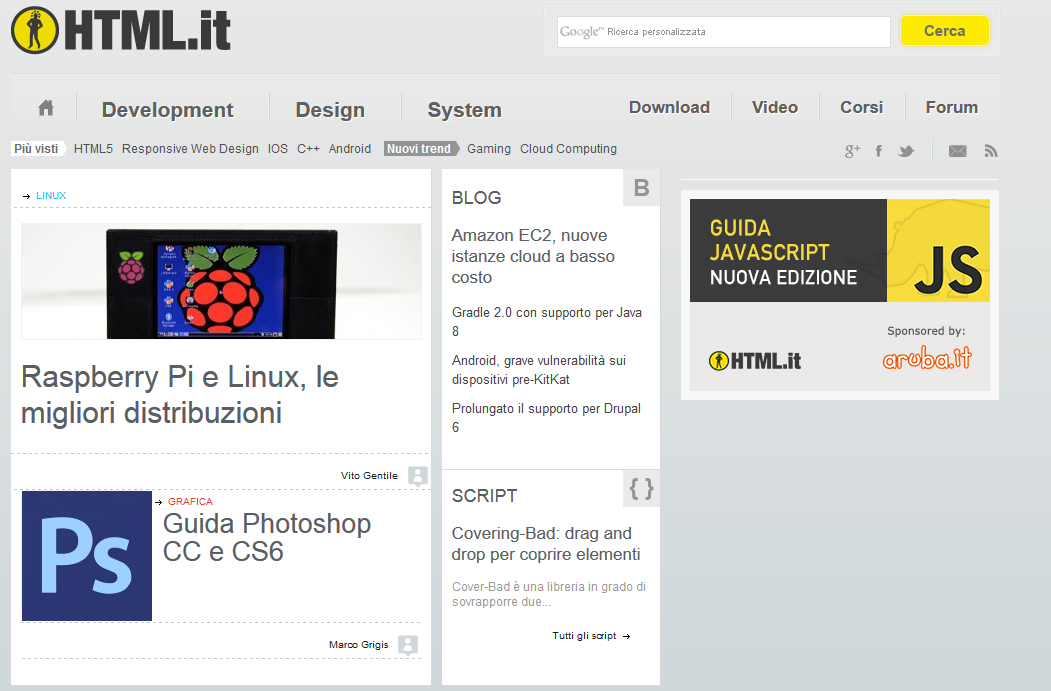
\includegraphics[width=120mm]{images/home.png}
\caption{La home page di html.it}
\end{figure}

Ho eseguito una serie di test ad una persona corrispondente al profilo indicato. Ho dato ad essa un tempo compreso tra i 10 e i 30 secondi e le ho detto di porsi le seguenti domande:

\subsection{Where?}

\begin{center}

\textit{``A che tipo di sito sono arrivato? Quale contenuto mi offre?''}

\end{center}

Il soggetto ha riconosciuto in tempi non eccessivamente lunghi che il sito si occupa di informatica e che offre la visualizzazione di articoli e guide. Ciò è stato possibile grazie alla presenza degli ultimi articoli direttamente nella home page. In questo modo è comprensibile a primo sguardo di cosa il sito tratta, per cui se il soggetto fosse stato interessato a leggere un articolo o una guida sull'argomento molto probabilmente avrebbe continuato la navigazione nel sito.

\subsection{Who?}

\begin{center}

\textit{``Chi rappresenta il sito?''}

\end{center}

Posso affermare con certezza che se il soggetto non avesse avuto la minima idea di cosa significassero termini come \textit{javascript}, \textit{raspberry} o \textit{photoshop} probabilmente ci avrebbe messo un tempo molto più alto, ragion per cui a mio modo di vedere per migliorare ques'aspetto una buona idea sarebbe quella di inserire uno slogan affianco al banner \textbf{html.it}. In questo modo a questa domanda si potrà rispondere in tempi brevissimi e inferiori ai 5 secondi, mentre allo stato attuale difficilmente si riesce a rispondere a primo impatto, ed è necessario dunque continuare la navigazione, obiettivo che è molto difficile da raggiungere.

\subsection{Why?}

\begin{center}

\textit{``Perchè mai dovrei fermarmi su questo sito? Quali benefici mi porta?''}

\end{center}

Il sito non presenta un'evidente pagina o sezione in cui viene descritto cosa esso rappresenta. Dà per scontato il fatto che il visitatore sappia esattamente dov'è arrivato e conosca precedentemente la sua fama. html.it è un sito molto rinomato, probabilmente chiunque lavora nel settore ci sarà capitato decine di volte. Ciononostante un buon sito web non può basarsi su questa supposizione, deve cercare di racchiudere nella sua cerchia il maggior numero di utenti possibili e dar loro un motivo per tornarci. In questo momento l'utente non ha un'idea molto chiara, non sa ancora se conviene soffermarsi oppure no.

Un sito web che si presenta bene ed esplicita in modo chiaro ciò che rappresenta porta all'utente un certo grado di fiducia. Come già detto prima una possibile miglioria sarebbe quella di inserire una breve descrizione nel banner e in aggiunta, a mio modo di vedere, una sezione in cui viene descritto il sito, i suoi componenti e i suoi scopi.

\subsection{What?}

\begin{center}

\textit{``Cosa offre il sito?''}

\end{center}

Supponiamo che l'utente sia stato colpito dalla home page e abbia deciso di restare per qualche minuto sul sito. A questo punto deciderà dunque di guardarsi intorno, scrollerà probabilmente verticalmente verso il basso e ciò che vedrà sarà la Figura ~\ref{fig:f3}.

\begin{figure}[H]
\centering
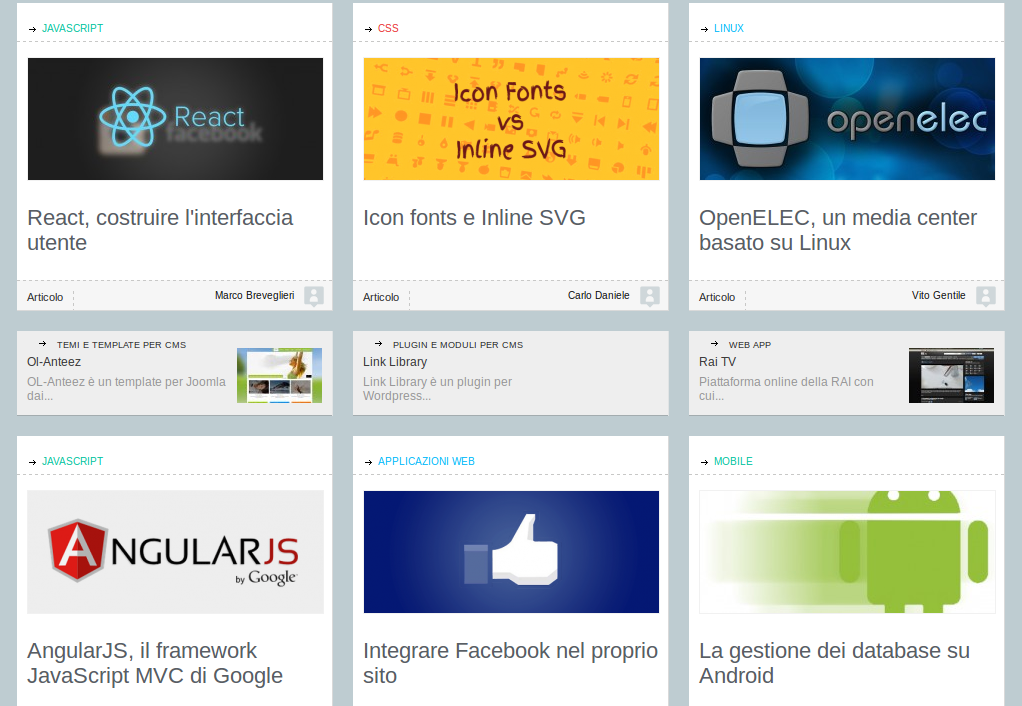
\includegraphics[width=120mm]{images/screen1.png}
\caption{La home page con uno scroll verso il basso}
\label{fig:f3}
\end{figure}

Come possiamo vedere troviamo tutta una serie di guide e articoli su diversi argomenti, il tutto disposto con visualizzazione a griglia. Questo è chiaramente un punto a favore, la visualizzazione a griglia è risultata (ed è tuttora) molto popolare negli ultimi anni, basti pensare alle interfacce di sistemi operativi come Android o iOS per gli smartphone o l'interfaccia Metro di Windows 8. L'avere un'interfaccia di questo tipo evita l'utente di scrollare troppo verso il basso per accedere ai contenuti e quindi lo stress è notevolmente diminuito. Ciascuno di questi ``mattoncini'' è cliccabile e il link rimanda alla relativa guida o articolo. La home page risponde quindi molto bene a questa domanda.

Una cosa molto fastidiosa però è rappresentata dalla figura seguente:

\begin{figure}[H]
\centering
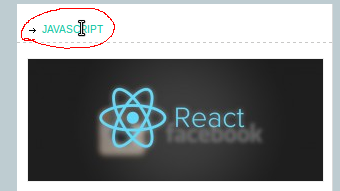
\includegraphics[width=50mm]{images/detail1.png}
\caption{Possibile link che non è un link}
\end{figure}

Ho segnato in rosso un difetto piuttosto rilevante. Chiunque vedendo l'articolo e la sua categoria si aspetta di cliccare sulla categoria ed essere rimandati ad una pagina contenente la lista degli ultimi articoli riguardanti quella categoria. Questo però non avviene e il possibile link è in realtà del semplice testo. Questo crea sicuramente frustrazione all'utente e fa chiaramente perdere i punti che il sito si era guadagnato con la visualizzazione a griglia.

\subsection{When?}

\begin{center}

\textit{``Quali sono le ultime novità? Quando è stato manutenuto per l'ultima volta?''}

\end{center}

Il sito risponde molto bene a questa domanda. Nella home page sono presenti gli ultimi articoli inseriti e ogni giorno è possibile scoprire i contenuti nuovi. Questo è importantissimo, perchè non c'è cosa peggiore di dare all'utente la sensazione di staticità. Se si vuol far sì che l'utente sia invogliato a tornare, bisogna fargli credere che quando tornerà per la seconda o terza o n-esima volta troverà sempre contenuti aggiornati e nuovi articoli o guide interessanti. Dare evidenza di manutenibilità di un sito web produce molta affidabilità e dà all'utente una fiducia non indifferente.



\subsection{How?}

\begin{center}

\textit{``Come faccio ad arrivare alle sezioni principali?''}

\end{center}

In questo caso il sito presenta un aspetto buono e uno non buono. Il fatto positivo è che la navigazione è tutto sommato ben strutturata. Come sottolineato nel precedente capitolo le guide e gli articoli si suddividono in tre categorie principali:

\begin{enumerate}

\item Development;
\item Design;
\item System.

\end{enumerate}

Il menu di navigazione evidenzia questi tre macro livelli e permette la navigazione al livello inferiore tramite un menu a tendina, come mostrato nella due figure seguenti:

\begin{figure}[H]
\centering
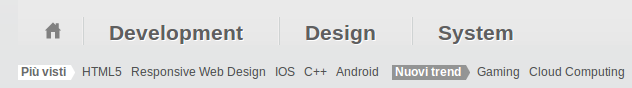
\includegraphics[width=120mm]{images/menu.png}
\caption{Menu di navigazione a tendina chiusa}
\end{figure}

\begin{figure}[H]
\centering
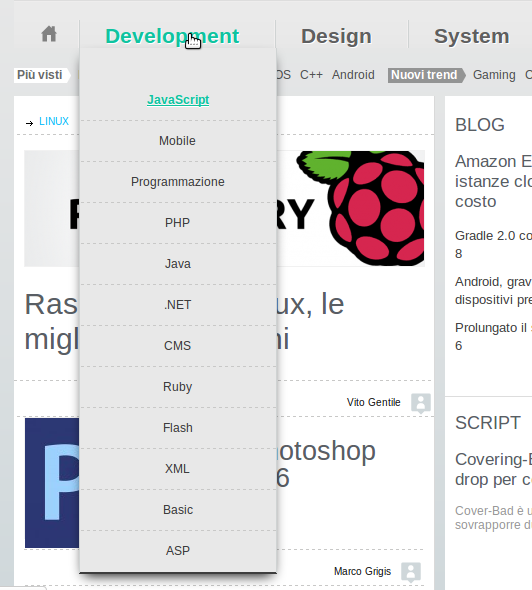
\includegraphics[width=80mm]{images/menu1.png}
\caption{Menu a di navigazione a tendina aperta}
\end{figure}

Il menu a tendina è facilmente navigabile ed è intuitivo, inoltre fa sì che il menu occupi poco spazio nell'intera pagina, dando più peso dunque al contenuto. Tramite questo menu l'utente può destreggiarsi all'interno del sito e raggiungere le sezioni a cui è interessato. Inoltre sotto al menu sono presenti i link alle guide e agli articoli più visitati, cosa sicuramente molto utile.

L'aspetto negativo è che da un lato il menu è poco visibile e non risalta all'occhio in modo immediato, mentre dall'altro nel momento in cui io scrollo verticalmente verso il basso esso sparisce, costringendomi a scrollare nuovamente verticalmente verso l'alto per tornare ad esso. Ora, questa è decisamente una mia opinione, ma credo che se si utilizzasse un menu fisso che risulta sempre visibile lungo tutta la navigazione si guadagnerebbe qualche punto in usabilità. Chiaramente può dare fastidio ed essere visivamente ingombrante. In tal caso una soluzione sarebbe ridurre lo spessore e renderlo simile alla barra di navigazione di facebook. Questa però è solamente la mia opinione.

